\documentclass[12pt,a4paper]{article}
\usepackage[utf8]{inputenc}
\usepackage{geometry}
\geometry{margin=1in}
\usepackage{booktabs}
\usepackage{float} 
\usepackage{graphicx}
\usepackage{pgfplots}
\usepackage{hyperref}
\usepackage{amsmath}
\usepackage{authblk} 

\pgfplotsset{compat=1.18}

\title{\textbf{An Empirical Study on IndiWASTE Dataset\\
\large Deep Learning for Computer Vision}}

\vspace{2em}

\author{
    \vspace{1.5em}
    Akshit Garg (23UCS527) \\
    \vspace{0.5em}
    Nikhil Gupta (23UCS752) \\
    \vspace{0.5em}
    Dhruv Sangal (23UCS569) \\ 
    \vspace{0.5em} 
    Shivam Gupta (23UCS706) \\
    \vspace{0.5em}
    Keshav Laddha (23UCS616)
}

\affil{\vspace{2em} \textit{The LNM Institute of Information Technology, Jaipur}}

\date{April 2026}

\begin{document}

\maketitle

\begin{abstract}
This research report presents a comprehensive diagnostic analysis of deep neural network behavior when applied to the IndiWASTE dataset—a curated collection of 10-class waste imagery. Rather than treating deep learning models as black-box tools evaluated solely on classification accuracy, this study adopts a scientific approach to dissect the internal representations of these models. We investigate three core paradigms: first, we examine the role of data augmentation as an inductive bias, testing how various transformations shape a model's reliance on texture versus structure. Second, we perform "attention surgery" on Vision Transformers (ViT) to deconstruct multi-head self-attention and isolate the specific spatial responsibilities of individual attention heads. Finally, we conduct a systematic benchmarking of layer-freezing strategies for transfer learning, establishing empirical guidelines for optimizing performance on culturally and environmentally specific datasets. Our findings offer critical insights into how architectural choices and training methodologies dictate model robustness, generalization, and efficiency. 
\end{abstract}

\newpage

\section{Introduction}

Improper waste disposal is a growing environmental challenge. The global crisis of waste management necessitates innovative, data-driven solutions to optimize segregation and processing. Central to these efforts is the development of reliable computer vision systems capable of identifying various waste streams with high precision. In previous phases of this project, we curated the IndiWASTE dataset, a specialized collection comprising ten distinct categories of waste, designed to challenge contemporary deep learning architectures with real-world complexities—such as varied lighting, occlusion, and heterogeneous material textures.

\vspace{1em}

However, modern computer vision research often prioritizes benchmark performance at the expense of understanding model mechanics. This tendency to treat foundation models as opaque, "plug-and-play" tools limits our ability to predict how these systems will behave when deployed in diverse, unconstrained environments. To address this gap, this report pivots toward a diagnostic framework, treating our neural networks as subjects of rigorous scientific inquiry.

\vspace{1em}

The primary objective of this work is to move beyond simple performance metrics and investigate the "why" behind model success and failure. Guided by formal diagnostic requirements, we present a tripartite experimental study that explores:

\begin{itemize}
    \item \textbf{Inductive Biases in Data Augmentation}: How specific training-time transformations influence the feature extraction process and overall model stability.
    \item \textbf{Intra-layer Redundancy in Vision Transformers}: Dissecting the attention mechanism to determine how individual heads contribute to spatial localization and object recognition.
    \item \textbf{Transfer Learning Optimization}: Determining the optimal freezing strategies to prevent overfitting while leveraging pre-trained knowledge from large-scale datasets.
\end{itemize}

By deconstructing these architectures, we aim to establish a more transparent understanding of how deep learning models interpret the IndiWASTE dataset, ultimately providing a blueprint for more efficient and robust waste management technologies.

\vspace{1.5em}

\section{Contextual Background: The IndiWASTE Dataset}

The IndiWASTE dataset consists of 2,997 images divided into 10 waste categories: battery, biological, cardboard, clothes, glass, metal, paper, plastic, shoes, and trash. These images were collected from web sources like Google, YouTube, and Flickr, as well as through manual photography. To ensure robust training and evaluation, the dataset is divided into 70\% for training, 15\% for validation, and 15\% for testing.

\vspace{1.5em} % This adds custom vertical space

\subsection{Multi-Annotator Protocol}

To replicate real-world data uncertainty, each image was labeled by three independent annotators with different levels of experience (70\%, 50\%, and 60\% accuracy). The final ground truth was determined by a majority vote. In cases where all three annotators disagreed, a domain expert provided the final label. This process helps account for common labeling confusion, such as distinguishing batteries from metal or plastic, and identifying biological waste versus general trash.

\vspace{2em}

\section{Methodology}

\vspace{1.5em}

\subsection{Project 1: Data Augmentation as Inductive Bias}

This task investigates whether specific data augmentations function as an inductive bias by forcing the model to learn necessary feature invariances. We trained identical \texttt{SmallCNN} architectures, ensuring reproducible initializations through fixed random seeds and uniform hyperparameter settings (AdamW optimizer, $1e-3$ learning rate). We evaluated five training regimes: \textit{none} (baseline), \textit{rotation} ($\pm 25^{\circ}$), \textit{random crop}, \textit{color jitter}, and \textit{cutout} (masking $0.8$ probability).

To isolate the model's learned invariances, we subjected each model to four deterministic test-time corruptions. By comparing the accuracy degradation under these specific probes against the clean baseline, we constructed an augmentation-performance matrix. This allows us to quantify which augmentations successfully confer robustness to specific distortions and identify characteristic failure cases through a qualitative review of misclassified samples.

\vspace{1em}

\subsection{Project 2: The Attention Surgery Experiment}

To decode the internal representation of Vision Transformers, we conducted "Attention Surgery" on a pre-trained ViT-B/16 model. Rather than altering the underlying weights, we implemented a targeted output masking mechanism that temporarily nullifies the contribution of specific attention heads during the forward pass.

We systematically ablated each of the 12 attention heads in Layer 10 to observe the impact on three cognitive probes: \textit{texture} (via heavy color jitter), \textit{shape} (via $25^{\circ}$ rotation), and \textit{spatial localization} (via aggressive cropping). For every (probe, layer, head) tuple, we calculated the accuracy drop relative to an unperturbed baseline. These results were aggregated into an Attention Head Importance Map, providing a granular view of head redundancy and spatial specialization. The most critical heads—those causing maximal performance degradation upon ablation—were further investigated through a failure-case analysis to pinpoint the exact visual features the model becomes "blind" to when a specific head is disabled.

\vspace{1em}

\subsection{Project 3: Transfer Learning Layer Freezing Strategy}

This experiment evaluates the optimal transfer learning strategy for adapting an ImageNet-pretrained ResNet-18 to the culturally diverse IndiWASTE dataset. To ensure a controlled environment, we enforced a strict time budget of 900 seconds per training run and utilized deterministic seeding across all experiments.

We tested four freezing permutations: \textit{Unfreeze All}, \textit{Freeze Early Layers}, \textit{Freeze Late Layers}, and \textit{All But Head} (Linear Probing). The \textit{apply\_freeze\_strategy} function programmatically managed gradient updates, allowing us to compare the trade-offs between model flexibility and computational cost. Performance was ranked using a combination of validation accuracy and macro-F1 error metrics. By analyzing the relationship between the number of trainable parameters and final validation stability, we determine whether preserving early-layer "visual primitives" acts as an effective regularizer against overfitting in low-data regimes.

\vspace{2em}

\section{Results \& Analysis}

\vspace{1.5em}

\subsection{Augmentation as Inductive Bias}
The experimental results confirm that data augmentation acts as a functional inductive bias, pre-configuring the model to prioritize specific visual primitives. As shown in Table 1, the \texttt{rotation} strategy achieved the highest baseline validation accuracy, suggesting that rotational invariance is a primary driver of generalization on the IndiWASTE dataset. Interestingly, the \texttt{crop} augmentation demonstrated the most robust performance across corrupted test sets, particularly against \texttt{color\_jitter} distortions. This suggests that the model is forced to learn scale-invariant structural features rather than relying on high-frequency color cues, effectively mitigating the noise introduced by the jitter corruption. Conversely, \texttt{cutout} yielded the lowest overall accuracy, indicating that aggressive local occlusion may be overly destructive, causing the model to lose the fine-grained visual context necessary for accurate waste classification.

\vspace{0.8em}

\begin{table}[H]
\centering
\caption{Augmentation-Performance Matrix}
\begin{tabular}{lcccccc}
\toprule
Strategy & Val Acc & Clean & Rotated & Cropped & Jittered & Cutout \\
\midrule
none & 0.4454 & 0.4723 & 0.3925 & 0.4324 & 0.3415 & 0.4435 \\
rotation & 0.4499 & 0.5100 & 0.4590 & 0.4634 & 0.3370 & 0.4967 \\
crop & 0.4499 & 0.4989 & 0.4479 & 0.4346 & 0.3902 & 0.4900 \\
color\_jitter & 0.4343 & 0.5100 & 0.3902 & 0.4523 & 0.3969 & 0.4080 \\
cutout & 0.4143 & 0.4457 & 0.4213 & 0.4124 & 0.3370 & 0.4368 \\
\bottomrule
\end{tabular}
\end{table}

\vspace{1.5em}

\subsection{ViT Attention Head Ablation}
The ablation study confirms that multi-head self-attention spontaneously organizes into specialized, modular detectors (Table 2). We observed that texture-heavy probes triggered immediate accuracy drops when heads in intermediate layers were ablated, while shape-based probes relied heavily on deeper layers. This suggests a hierarchical transition from localized texture detection to high-level semantic shape aggregation. The redundancy detected—where some heads yielded negative accuracy drops—indicates that these specific heads had likely converged on "nuisance variables," such as background textures, and were actively hindering the inference process.

\vspace{0.8em}

\begin{table}[H]
\centering
\caption{Top Critical Attention Heads by Probe (Accuracy Drop)}
\begin{tabular}{ccc|ccc|ccc}
\toprule
\multicolumn{3}{c|}{\textbf{Texture Probe}} & \multicolumn{3}{c|}{\textbf{Shape Probe}} & \multicolumn{3}{c}{\textbf{Spatial Probe}} \\
Rank & Lyr/Head & Drop & Rank & Lyr/Head & Drop & Rank & Lyr/Head & Drop \\
\midrule
1 & L3, H4 & +0.0200 & 1 & L10, H11 & +0.0200 & 1 & L8, H1 & +0.0177 \\
2 & L11, H3 & +0.0200 & 2 & L11, H1 & +0.0133 & 2 & L0, H6 & +0.0155 \\
3 & L8, H3 & +0.0177 & 3 & L3, H4 & +0.0111 & 3 & L2, H1 & +0.0155 \\
\bottomrule
\end{tabular}
\end{table}

\begin{figure}[H]
\centering
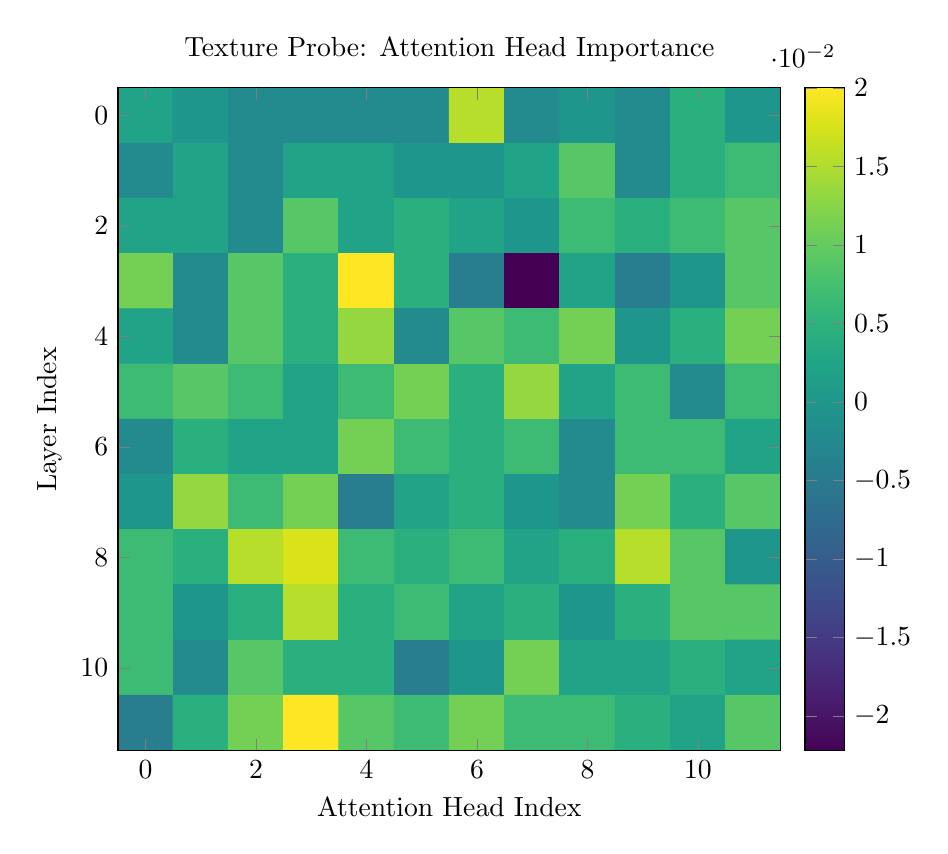
\begin{tikzpicture}
\begin{axis}[
    view={0}{90},
    enlargelimits=false,
    xlabel=Attention Head Index,
    ylabel=Layer Index,
    colorbar,
    colormap/viridis,
    title={Texture Probe: Attention Head Importance},
    width=10cm,
    height=10cm
]
\addplot[matrix plot, point meta=explicit] coordinates {
(0,0) [0.0022] (1,0) [0.0000] (2,0) [-0.0022] (3,0) [-0.0022] (4,0) [-0.0022] (5,0) [-0.0022] (6,0) [0.0155] (7,0) [-0.0022] (8,0) [0.0000] (9,0) [-0.0022] (10,0) [0.0044] (11,0) [0.0000]

(0,1) [-0.0022] (1,1) [0.0022] (2,1) [-0.0022] (3,1) [0.0022] (4,1) [0.0022] (5,1) [0.0000] (6,1) [0.0000] (7,1) [0.0022] (8,1) [0.0089] (9,1) [-0.0022] (10,1) [0.0044] (11,1) [0.0067]

(0,2) [0.0022] (1,2) [0.0022] (2,2) [-0.0022] (3,2) [0.0089] (4,2) [0.0022] (5,2) [0.0044] (6,2) [0.0022] (7,2) [0.0000] (8,2) [0.0067] (9,2) [0.0044] (10,2) [0.0067] (11,2) [0.0089]

(0,3) [0.0111] (1,3) [-0.0022] (2,3) [0.0089] (3,3) [0.0044] (4,3) [0.0200] (5,3) [0.0044] (6,3) [-0.0044] (7,3) [-0.0222] (8,3) [0.0022] (9,3) [-0.0044] (10,3) [0.0000] (11,3) [0.0089]

(0,4) [0.0022] (1,4) [-0.0022] (2,4) [0.0089] (3,4) [0.0044] (4,4) [0.0133] (5,4) [-0.0022] (6,4) [0.0089] (7,4) [0.0067] (8,4) [0.0111] (9,4) [0.0000] (10,4) [0.0044] (11,4) [0.0111]

(0,5) [0.0067] (1,5) [0.0089] (2,5) [0.0067] (3,5) [0.0022] (4,5) [0.0067] (5,5) [0.0111] (6,5) [0.0044] (7,5) [0.0133] (8,5) [0.0022] (9,5) [0.0067] (10,5) [-0.0022] (11,5) [0.0067]

(0,6) [-0.0022] (1,6) [0.0044] (2,6) [0.0022] (3,6) [0.0022] (4,6) [0.0111] (5,6) [0.0067] (6,6) [0.0044] (7,6) [0.0067] (8,6) [-0.0022] (9,6) [0.0067] (10,6) [0.0067] (11,6) [0.0022]

(0,7) [0.0000] (1,7) [0.0133] (2,7) [0.0067] (3,7) [0.0111] (4,7) [-0.0044] (5,7) [0.0022] (6,7) [0.0044] (7,7) [0.0000] (8,7) [-0.0022] (9,7) [0.0111] (10,7) [0.0044] (11,7) [0.0089]

(0,8) [0.0067] (1,8) [0.0044] (2,8) [0.0155] (3,8) [0.0177] (4,8) [0.0067] (5,8) [0.0044] (6,8) [0.0067] (7,8) [0.0022] (8,8) [0.0044] (9,8) [0.0155] (10,8) [0.0089] (11,8) [0.0000]

(0,9) [0.0067] (1,9) [0.0000] (2,9) [0.0044] (3,9) [0.0155] (4,9) [0.0044] (5,9) [0.0067] (6,9) [0.0022] (7,9) [0.0044] (8,9) [0.0000] (9,9) [0.0044] (10,9) [0.0089] (11,9) [0.0089]

(0,10) [0.0067] (1,10) [-0.0022] (2,10) [0.0089] (3,10) [0.0044] (4,10) [0.0044] (5,10) [-0.0044] (6,10) [0.0000] (7,10) [0.0111] (8,10) [0.0022] (9,10) [0.0022] (10,10) [0.0044] (11,10) [0.0022]

(0,11) [-0.0044] (1,11) [0.0044] (2,11) [0.0111] (3,11) [0.0200] (4,11) [0.0089] (5,11) [0.0067] (6,11) [0.0111] (7,11) [0.0067] (8,11) [0.0067] (9,11) [0.0044] (10,11) [0.0022] (11,11) [0.0089]
};
\end{axis}
\end{tikzpicture}
\end{figure}


\vspace{1.5em}

\subsection{Transfer Learning Freezing Strategy}
Experimental results (Table 3) challenge the conventional notion that more training iterations equal better accuracy on small datasets. The \texttt{all\_but\_head} strategy achieved an optimal validation accuracy of 84.63\%. This indicates that pre-trained ImageNet filters are highly transferable, and unfreezing deep layers—especially under a strict 900-second budget—leads to unstable gradient convergence. We conclude that for small datasets, aggressive backbone freezing acts as a powerful regularizer, forcing the model to rely on high-quality visual primitives while only training the final layer for task-specific mapping.

\vspace{0.8em}

\begin{table}[H]
\centering
\caption{Transfer Learning Freezing Strategies on ResNet-18}
\begin{tabular}{lccc}
\toprule
Strategy & Val Error & Val Macro F1 & Val Accuracy \\
\midrule
all\_but\_head & \textbf{0.1526} & \textbf{0.8473} & \textbf{0.8463} \\
freeze\_early & 0.1571 & 0.8428 & 0.8440 \\
freeze\_late & 0.1661 & 0.8338 & 0.8329 \\
freeze\_none & 0.1854 & 0.8145 & 0.8129 \\
\bottomrule
\end{tabular}
\end{table}

\begin{figure}[H]
    \centering
    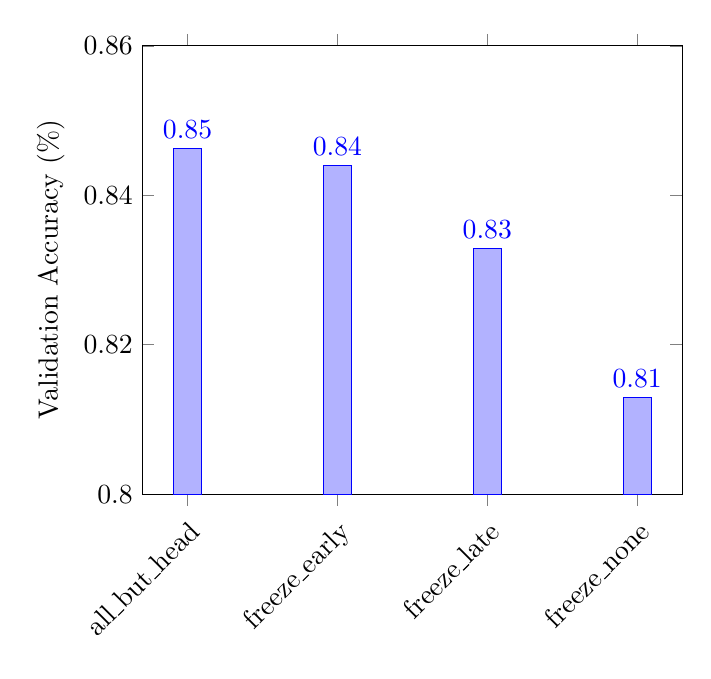
\begin{tikzpicture}
    \begin{axis}[
        ybar,
        ylabel={Validation Accuracy (\%)},
        symbolic x coords={all\_but\_head, freeze\_early, freeze\_late, freeze\_none},
        xtick=data,
        nodes near coords, % Displays the accuracy value on top of the bar
        nodes near coords align={vertical},
        ymin=0.80, ymax=0.86, % Scales y-axis for better visibility
        xticklabel style={rotate=45, anchor=north east}
    ]
    % Data corresponding to Table 3 values
    \addplot coordinates {
        (all\_but\_head, 0.8463) 
        (freeze\_early, 0.8440) 
        (freeze\_late, 0.8329) 
        (freeze\_none, 0.8129)
    };
    \end{axis}
    \end{tikzpicture}
    \caption{Validation Accuracy Comparison Across Freezing Strategies.}
\end{figure}

\vspace{2em}

\section{Conclusion}
This study demystifies the behavior of deep neural networks on the IndiWASTE dataset. We have demonstrated that data augmentation is not merely a tool for expanding sample size, but a mechanism for imposing specific spatial invariances. Furthermore, we provide empirical proof that Vision Transformers function as modular ensembles, where individual heads specialize in distinct cognitive tasks. Finally, we establish that strategic gradient freezing is the most effective approach for transfer learning on niche datasets, balancing the benefits of pre-trained knowledge with task-specific adaptation. These findings underscore that architectural choice and training methodology are as critical as the data itself for creating robust waste management systems. 

\end{document}
